\chapter{Clean Architecture}
In diesem Kapitel steht die Clean Architecture und deren zentrale Aspekte im Fokus. Zuerst erfolgt eine Analyse der Dependency Rule, einer Schlüsselregel der Clean Architecture. Untersucht werden dabei die Auswirkungen dieser Regel auf die Softwarearchitektur, ergänzt durch positive und negative Anwendungsbeispiele.

Im Anschluss daran richtet sich der Fokus auf die Struktur der Clean Architecture, wobei die einzelnen Schichten detailliert analysiert werden. Besondere Aufmerksamkeit gilt dabei den Schichten "Domain" und "Application", deren Rolle und Bedeutung innerhalb der Clean Architecture ausführlich diskutiert werden. Diese Analysen ermöglichen ein tiefgreifendes Verständnis der Clean Architecture und ihrer praktischen Anwendung.
\section{Was ist Clean Architecture}
Die \textbf{Clean Architecture}, auch bekannt als die \textbf{Onion Architecture}, ist ein Software-Entwurfsprinzip, das von Robert C. Martin, entwickelt wurde. Sie zielt darauf ab, eine klare und getrennte Struktur in Software-Systemen zu schaffen, um Wartbarkeit, Testbarkeit und Flexibilität zu verbessern und somit den Rahmen für eine effiziente und zukunftssichere Softwareentwicklung zu schafft.\\

Die Struktur der Clean Architecture teilt eine Anwendung in konzentrische Schichten auf. Jede Schicht erfüllt bestimmte Arten von Aufgaben und weist klar definierte Abhängigkeiten auf. Dies ist ein entscheidender Aspekt, um eine hohe Entkopplung und Kohäsion innerhalb des Systems zu erreichen. Von innen nach außen sind die Schichten wie folgt strukturiert:

\begin{figure}[ht]
    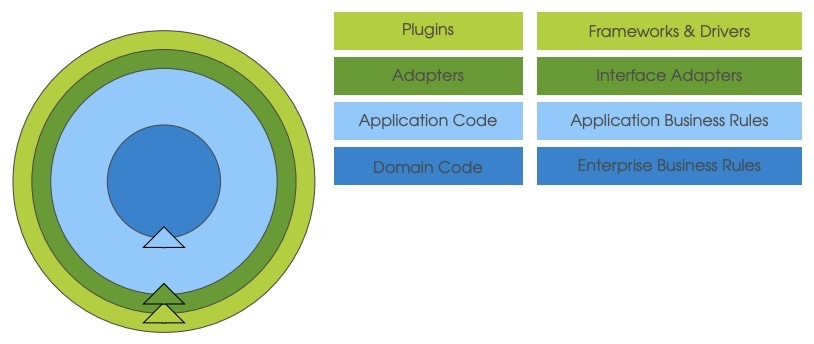
\includegraphics[width=1\textwidth]{Bilder/clean-architecture.jpeg}
    \caption{Clean Architecture Schichten\cite{briem}}
    \label{fig:clean-architecture}
\end{figure}
\newpage
\textbf{Domain-Schicht}: Die innerste Schicht, die die Geschäftslogik und Geschäftsregeln einer Anwendung enthält. Sie hat keine Abhängigkeiten von den äußeren Schichten und repräsentiert die fundamentalen Konzepte der Anwendung, unabhängig von spezifischen technologischen Details. Die Unabhängigkeit dieser Schicht ermöglicht eine hohe Testbarkeit und Flexibilität.

\textbf{Anwendungs-Schicht}: Diese Schicht enthält spezifische Geschäftslogik, die sich auf bestimmte Anwendungsfälle bezieht. Sie ist von der Domain-Schicht abhängig und kann mit ihr interagieren, kennt aber keine Details über äußere Schichten. Die Anwendungsschicht orchestriert die Interaktion zwischen der Domain-Schicht und den äußeren Schichten und stellt so eine Trennung der Belange sicher.

\textbf{Adapter-Schicht}: Sie dient der Übersetzung von Daten zwischen den für die inneren und äußeren Schichten geeigneten Formaten. Sie kann Datenbankcode, Benutzeroberflächen-Code oder sogar Code für externe Dienste enthalten. Sie fungiert als Brücke zwischen der inneren Logik und der Außenwelt.

\textbf{Plugin-Schicht}: Die äußerste Schicht, die spezifische Technologien wie Datenbanken, Webserver oder Frameworks umfasst. Sie interagiert mit den inneren Schichten durch Ports und Adapter. Diese Architektur ermöglicht eine einfache Ersetzbarkeit und Erweiterung von technologischen Komponenten.\\

Zusammenfassend lässt sich sagen, dass die Clean Architecture ein Ansatz ist, der darauf abzielt, die Unordnung und Komplexität in Softwareprojekten zu reduzieren, indem klare Grenzen und Regeln für die Struktur und Organisation des Codes vorgegeben werden. Sie ermöglicht es Entwicklern, Systeme zu erstellen, die widerstandsfähig gegenüber technologischen Änderungen sind und die sich im Laufe der Zeit leicht anpassen und erweitern lassen.
\section{Analyse der Dependency Rule}
Die Dependency Rule ist das zentrale Prinzip der Clean Architecture und bestimmt die Richtung der Abhängigkeiten zwischen den verschiedenen Schichten. Sie besagt, dass Abhängigkeiten immer von den äußeren Schichten zu den inneren Schichten gerichtet sein sollten, was bedeutet, dass der Code in den inneren Schichten frei von spezifischen technologischen Implementierungsdetails bleiben kann.

In der Praxis führt diese Regel dazu, dass der Code in den inneren Schichten unabhängig von spezifischen Technologien in den äußeren Schichten entwickelt und getestet werden kann. Dies erleichtert die Wartung des Codes und ermöglicht eine höhere Testabdeckung, da die Geschäftslogik unabhängig von spezifischen Technologien getestet werden kann.

Darüber hinaus fördert die Dependency Rule die Entkopplung der Schichten und trägt zur Flexibilität des Systems bei. Durch die eindeutige Trennung der Verantwortlichkeiten und die Richtung der Abhängigkeiten können Änderungen in den äußeren Schichten vorgenommen werden, ohne die inneren Schichten zu beeinflussen. Das System bleibt dadurch anpassungsfähig und widerstandsfähig gegenüber technologischen Änderungen.

Die Dependency Rule unterstützt auch die Anwendung der SOLID-Prinzipien, insbesondere das \acf{SRP} und das \acf{OCP}. Durch die klare Trennung der Verantwortlichkeiten zwischen den Schichten können diese ihre spezifischen Aufgaben erfüllen und gleichzeitig offen für Erweiterungen, aber geschlossen für Modifikationen bleiben. Dies führt zu einer verbesserten Modularität und Austauschbarkeit der Komponenten.

Abschließend kann man sagen, dass die Dependency Rule nicht nur dazu beiträgt, die Wartbarkeit und Testbarkeit der Software zu verbessern, sondern auch eine klare und verständliche Struktur in der Codebasis fördert. Sie trägt zur Reduzierung der Komplexität bei, indem sie klare Grenzen und Regeln für die Struktur und Organisation des Codes vorgibt.

Die Clean Architecture und ihre Dependency Rule zielen insgesamt darauf ab, die Langlebigkeit und Widerstandsfähigkeit von Softwareprojekten zu verbessern. Sie ermöglicht es Entwicklern, Systeme zu erstellen, die sich an verändernde Anforderungen und Technologien anpassen können, ohne dass umfangreiche Überarbeitungen erforderlich sind. Durch die klare Strukturierung und Organisation des Codes können Entwickler effizienter arbeiten und gleichzeitig die Qualität ihrer Software sicherstellen.

Zusammenfassend lässt sich sagen, dass die Clean Architecture und insbesondere die Dependency Rule wesentliche Bestandteile einer modernen und zukunftssicheren Softwareentwicklung sind. Sie bieten Entwicklern ein solides Fundament, auf dem sie hochwertige, wartbare und flexible Softwarelösungen erstellen können, die den Anforderungen von heute und morgen gerecht werden.\\

Im Folgenden werden zwei Beispiele für die Einhaltung der Dependency Rule gezeigt.
\section{Positiv-Beispiel: Dependency Rule}
Im Projekt wurden die unterschiedlichen Schichten der Clean Architecture mit Modulen realisiert, welche von Maven verwaltet werden. Das hat den Vorteil, dass die inneren Schichten nicht auf die äußeren Schichten zugreifen können, sofern dieses Verhalten nicht explizit definiert ist.
\begin{figure}[ht]
    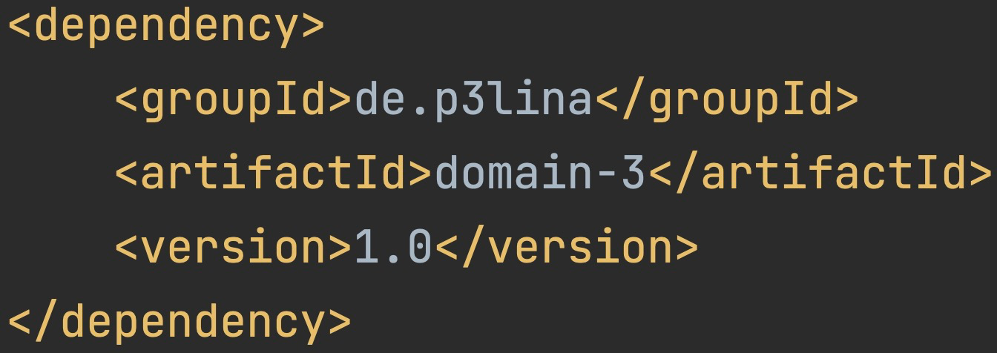
\includegraphics[width=0.7\textwidth]{Bilder/pom_application.png}
    \caption{POM Application layer}
    \label{fig:pom-application}
\end{figure}
\begin{figure}[ht]
    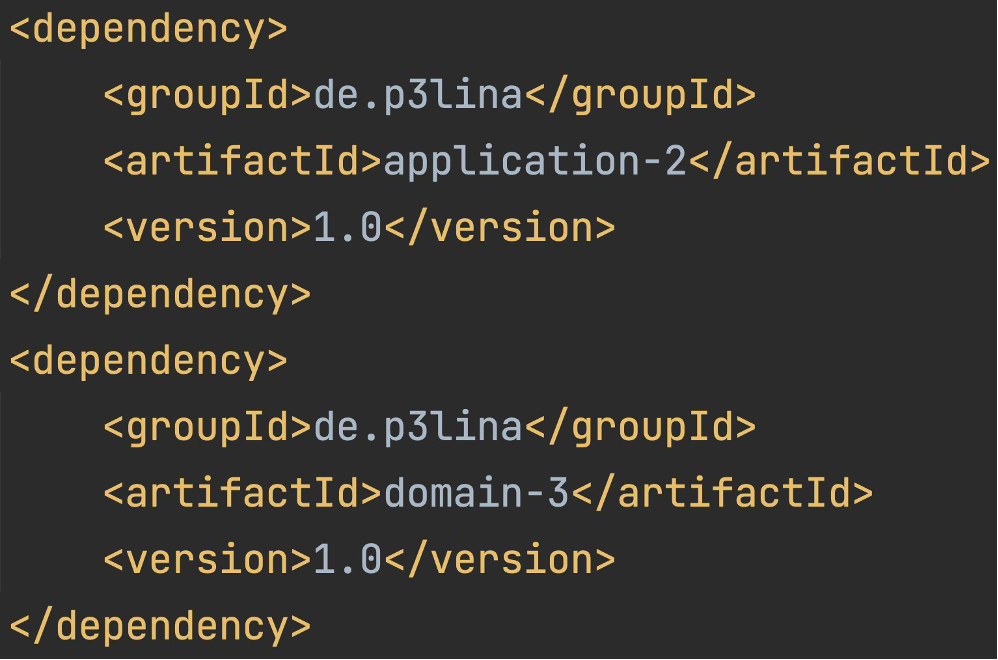
\includegraphics[width=0.7\textwidth]{Bilder/pom_adapters.png}
    \caption{POM Adapters layer}
    \label{fig:pom-adapters}
\end{figure}\\
In diesen beiden Code Ausschnitten ist zu sehen, wie die anderen Schichten in den Modulen importiert werden. \\Die Application Schicht importiert ausschließlich die Domain Schicht, da nur die Domain Schicht weiter innen im Schichtenmodell ist.\\
Die Adapters Schicht importiert die Application Schicht und die Domain Schicht.\newpage
\begin{figure}[ht]
    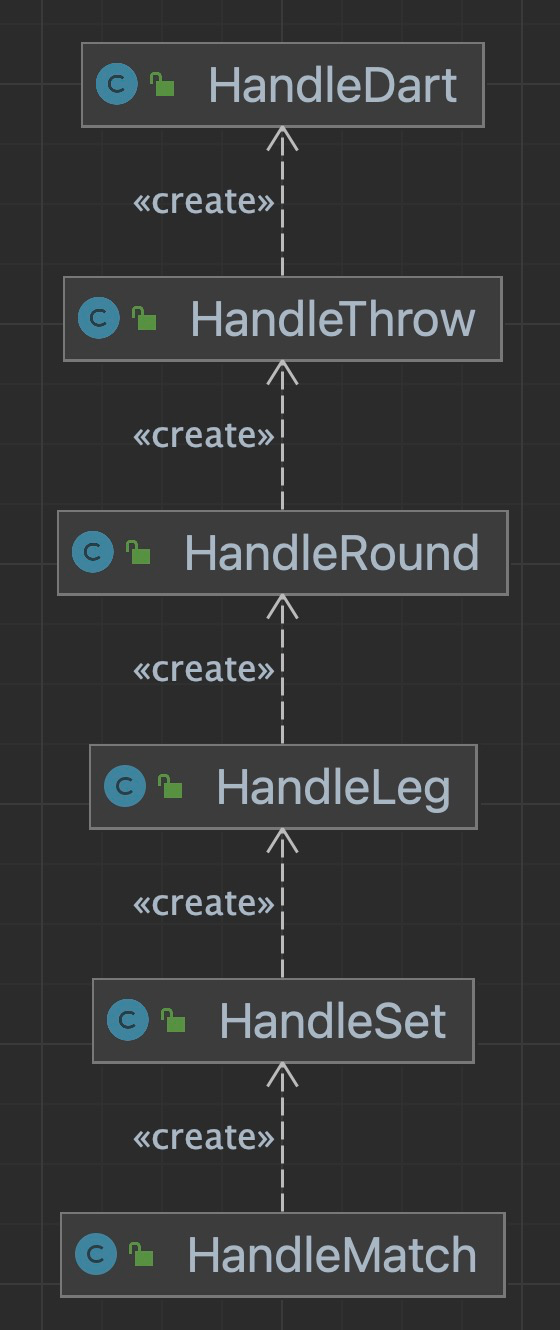
\includegraphics[width=0.3\textwidth]{Bilder/handleDiagram.png}
    \caption{Dart Game Handlers}
    \label{fig:dart-handlers}
\end{figure}
Als positiv Beispiel können die Handle Klassen für ein Dart Spiel verwendet werden. Diese dienen zum Verwalten der unterschiedlichen Teile eines Dart Spiels. Das Verhalten der Klassen ist prinzipiell immer gleich:\\
Die Klassen HandleMatch, HandleSet und HandleLeg bilden eine Struktur zur Organisation eines Dartspiels. Sie repräsentieren verschiedene Phasen des Spiels und sind für das Verwalten dieser Phasen zuständig.\\

HandleMatch ist für die Gesamtstruktur des Spiels verantwortlich. Sie erstellt ein Match-Objekt, das das gesamte Spiel repräsentiert. Während des Spiels wird jedes einzelne Set, das gespielt wird, von der HandleMatch Klasse an das Match-Objekt angefügt.\\

Diese Sets werden jedoch nicht direkt von HandleMatch erstellt. Stattdessen wird die Arbeit an die HandleSet-Klasse delegiert. HandleSet erstellt ein Set und verarbeitet alle damit verbundenen Daten. Jedes gespielte Leg, ein kleinerer Abschnitt innerhalb des Sets, wird von HandleSet zum Set-Objekt hinzugefügt.\\

Bevor das Leg jedoch zum Set hinzugefügt wird, wird es von der HandleLeg-Klasse verarbeitet. HandleLeg ist dafür zuständig, ein Leg zu erstellen und zu verwalten.\\

Die Struktur geht noch tiefer: Jedes Leg besteht aus mehreren Runden, die von der HandleRound-Klasse verwaltet werden. HandleRound erstellt und verwaltet eine Runde, in der mehrere Würfe, sogenannte Throws, stattfinden können. Jeder dieser Throws wird von der HandleThrow-Klasse erstellt und verwaltet.\\

Schließlich kommt die HandleDart-Klasse ins Spiel. Sie kümmert sich um die tatsächlichen Würfe mit dem Dart, den kleinsten Einheiten im Spiel.\\

So entsteht eine klare Hierarchie und Struktur: Ein Match besteht aus mehreren Sets, die aus mehreren Legs bestehen. Jedes Leg beinhaltet mehrere Runden und in jeder Runde werden mehrere Würfe, also Throws, durchgeführt. Jeder einzelne Wurf mit dem Dart wird auch verwaltet. Jede dieser Ebenen wird von einer eigenen Handle-Klasse verwaltet. Durch diese strukturierte Aufteilung ist es möglich, ein Dart-Spiel effizient und organisiert zu verwalten.\\
Diese Klassen liegen in der Application Scchicht und erstellen jeweils nur Objekte von Klassen der selben Schicht, womit die Dependency Rule eingehalten wird.
\section{Positiv-Beispiel: Dependency Rule}
\begin{figure}[ht]
    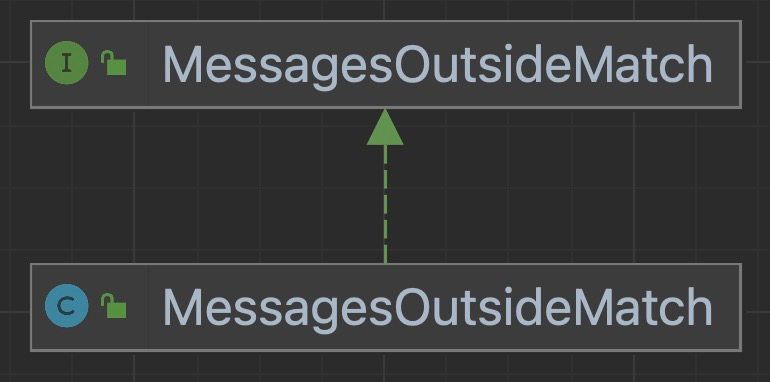
\includegraphics[width=0.3\textwidth]{Bilder/adapters_domain_uml.png}
    \caption{Adapters und Domain Class in UML}
    \label{fig:adapters-domain-uml}
\end{figure}
In diesem Beispiel nutzt eine Klasse in der Adapter-Schicht ein Interface aus der Domain-Schicht. Dies ermöglicht es beispielsweise der Anwendungsschicht, ein Objekt dieser Klasse aus der Adapter-Schicht zu übergeben, da die Anwendungsschicht das Interface aus der Domain-Schicht kennt.
\\
Der Vorteil dieser Vorgehensweise besteht darin, dass die Adapter-Schicht und die Domain-Schicht über das gemeinsame Interface miteinander kommunizieren können. Dadurch wird die Trennung zwischen den verschiedenen Schichten gewahrt und die Abhängigkeiten zwischen ihnen werden reduziert.
\\
In der Anwendungsschicht kann ein Objekt der Adapter-Klasse erzeugt werden, da die Anwendungsschicht das Interface aus der Domain-Schicht kennt. Dies ermöglicht eine flexible Handhabung der Klassen und erleichtert die Integration von Komponenten aus verschiedenen Schichten.
\section{Analyse der Schichten}
In diesem Abschnitt werden 2 Klassen aus den jeweiligen Schichten analysiert.
\subsection{Schicht: Domain}
\begin{figure}[ht]
    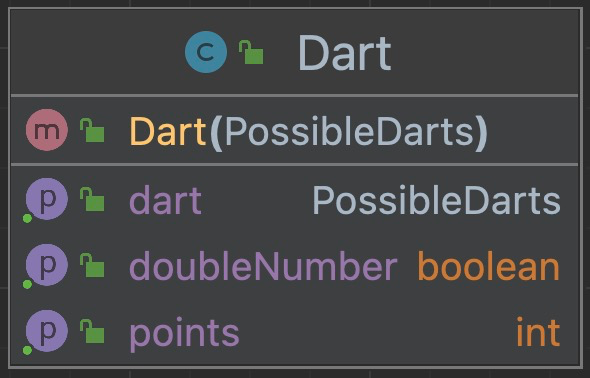
\includegraphics[width=0.5\textwidth]{Bilder/Dart.png}
    \caption{Dart Klasse der Domain Schicht}
    \label{fig:dart-uml}
\end{figure}
Die Dart Klasse ist eine Klasse der Domain Schicht. Sie enthält die Attribute \textit{dart} des Typs \textit{PossibleDarts}, \textit{doubleNumber} des Typs \textit{boolean} und \textit{points} des Typs \textit{int}. Erstellt werden kann ein Dart-Objekt mit Hilfe eines \textit{PossibleDarts}-Wertes. \textit{PossibleDarts} ist ein Enum der selben Schicht, welches alle möglichen Dart-Würfe enthält, zusammen mit der Punkt-Anzahl, die dieser Wurf erzielt und der Information, ob dieser Wurf ein Doppel ist oder nicht, da dies relevant für den Checkout ist.\\
Diese Klasse befindet sich in der Domain Schicht, da sie ein zentraler Bestandteil eines Dart-Spiels ist, von fast allen Schichten gekannt werden muss und sich deutlich seltener ändert als Klassen der anderen Schichten.
\subsection{Schicht: Application}
\begin{figure}[ht]
    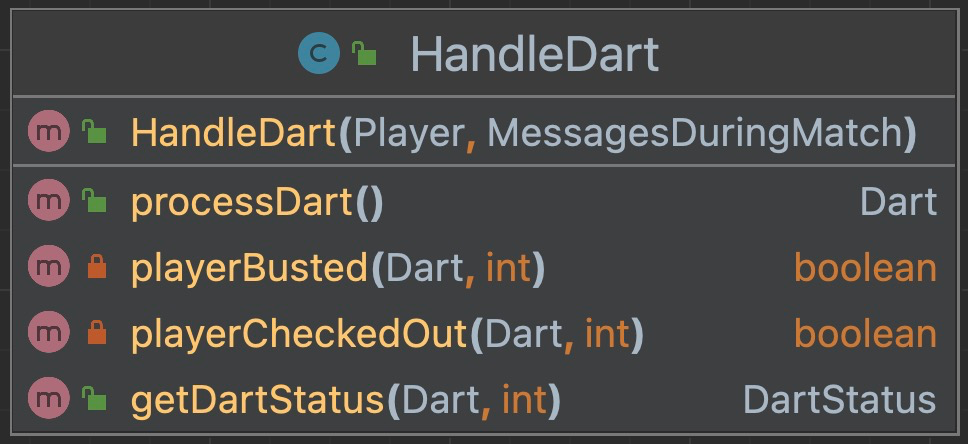
\includegraphics[width=0.5\textwidth]{Bilder/HandleDart.png}
    \caption{HandleDart Klasse der Application Schicht}
    \label{fig:handle-dart-uml}
\end{figure}
Diese Klasse der Application-Schicht dient zum Verwalten eines Dart-Wurfes. Das Herzstück dieser Klasse ist die \textit{processDart}-Methode. Diese wird vom überliegenden Teil des Dart Spiels, in diesem Fall der HandleThrow-Klasse oder genauer, der \textit{processThrow}-Methode, aufgerufen und gibt ein Objekt der Dart-Klasse aus der Domain-Schicht zurück.\\
Die anderen Methoden der Klasse dienen dazu, einen Spezialfall abzuprüfen, nämlich ob der Wurf eines Spielers ein checkout ist oder ob er damit überworfen (\textit{engl. busted}) hat.\\
Diese Klasse befindet sich in der Application-Schicht, da sie genau Regeln des Ablaufes eines Dart-Spiels implementiert. Solche Regeln können öfter geändert, angepasst und erweitert werden, weshalb diese Klasse in der Application-Schicht liegt.